\documentclass[11pt,a4paper]{article}
\usepackage[T1]{fontenc}
\usepackage[margin=2.3cm]{geometry}
\usepackage{amsmath,amssymb}
\usepackage{graphicx}
\usepackage[dvipsnames]{xcolor}
\usepackage{enumitem}
\usepackage[colorlinks=true,linkcolor=blue,urlcolor=blue]{hyperref}
\setlength{\parskip}{0.6em}
\setlength{\parindent}{0pt}
\begin{document}

\begin{center}{\LARGE\bfseries opentolerance}\\[0.4em]{\large Choose fits and tolerances so parts assemble and still work, in three sessions.}\\[0.2em]\small PAN IIT OSS explainer \textbullet{} diploma / undergraduate to advanced undergraduate (levels 5-6)\end{center}

\section*{Why this exists}
Every manufactured part differs a little from its drawing. This explainer shows how engineers describe that difference with limits, tolerance and fits, and how the differences of many parts add up in an assembly, using only subtraction, square roots and a bell curve.

\section*{The end goal}
Choose fits and tolerances so parts assemble and still work. The end goal is to choose fits and tolerances so that parts assemble and still work: tight enough to function, loose enough to be made at a sensible cost. The same ideas appear in machine design, electronics, optics and quality control.

\section*{How the three sessions build up}
\begin{enumerate}[nosep]
\item \textbf{Session 1: No part is made exactly: limits and tolerance} (Level 1, conceptual interactive model, 60 min).
\item \textbf{Session 2: ISO fits and the worst-case stack} (Level 2, mathematical engineering model, 75 min).
\item \textbf{Session 3: Statistical stack-up, capability and cost} (Level 3, simulation and validation, 90 min).
\end{enumerate}

\section{Session 1: No part is made exactly: limits and tolerance}

\subsection*{A. Real-world problem}
A shaft that is a little too big will not go into a hole that is a little too small. A machine cannot cut a hole to exactly 10.000 mm: tools wear, metal warms up, measuring has its own error. So the drawing does not say 'make it 10 mm'; it says 'make it between these two sizes'. How wide may that range be so that every pin still goes into every hole, and how much does a narrower range cost? Today we only ask the first half.

\subsection*{B. Concept and theory}
A part has an upper limit (the largest size allowed) and a lower limit (the smallest). The tolerance is the difference between them: the total wiggle we accept. A measured part is in tolerance if its size lies between the limits, and a size exactly on a limit is still acceptable. A pin goes into a hole if the hole is bigger than the pin. The clearance is the hole size minus the pin size. If the clearance is positive it is a clearance; if negative it is called interference (the pin is bigger than the hole); zero is line to line. When both parts may be anywhere inside their limits, the smallest clearance occurs with the biggest pin in the smallest hole and the largest clearance with the smallest pin in the biggest hole. In this session the pin is specified between 9.98 - tol and 9.98 mm and the hole between 10.00 and 10.00 + tol mm, where tol is the tolerance of each part.

\begin{itemize}[nosep]
\item upper, lower: upper and lower limits of a part (mm)
\item tol: tolerance = upper limit - lower limit (mm)
\item c: clearance = hole size - pin size (mm)
\item c\_min, c\_max: smallest and largest clearance over all allowed parts (mm)
\end{itemize}

\begin{equation*}
t = U - L
\end{equation*}

\begin{equation*}
c = d_{\mathrm{hole}} - d_{\mathrm{pin}}
\end{equation*}

\begin{equation*}
c_{\min} = L_{\mathrm{hole}} - U_{\mathrm{pin}},\qquad c_{\max} = U_{\mathrm{hole}} - L_{\mathrm{pin}}
\end{equation*}

\begin{center}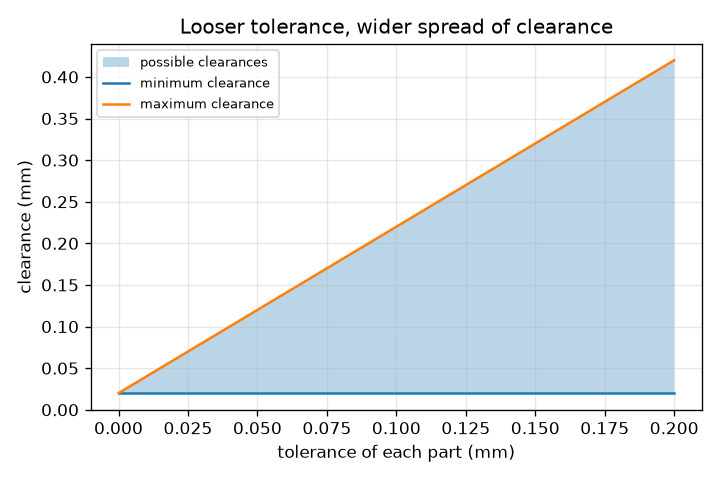
\includegraphics[width=0.85\linewidth]{figures/s01_clearance_vs_tol.png}\\\small The band of possible clearances widens as the tolerance of each part grows.\end{center}

\subsection*{E. Worked example}
With a tolerance of 0.05 mm on both parts, find the limits of the pin and of the hole, the smallest and largest clearance, and decide whether a pin measured at 9.99 mm is acceptable.
\begin{enumerate}[nosep]
\item Pin limits: upper 9.98 mm, lower 9.98 - 0.05 = 9.93 mm. Hole limits: lower 10.00 mm, upper 10.00 + 0.05 = 10.05 mm.
\item Tolerance of the pin = 9.98 - 9.93 = 0.05 mm, of the hole = 10.05 - 10.00 = 0.05 mm.
\item Smallest clearance = hole lower limit - pin upper limit = 10.00 - 9.98 = 0.02 mm.
\item Largest clearance = hole upper limit - pin lower limit = 10.05 - 9.93 = 0.12 mm.
\item A pin of 9.99 mm is above the upper limit 9.98 mm, so it is out of tolerance and is rejected, although it would still fit a 10.00 mm hole with 0.01 mm to spare. The drawing, not the single fit, decides.
\end{enumerate}
\textbf{Answer.} Clearance 0.02 to 0.12 mm for every allowed pin and hole; the 9.99 mm pin is rejected.

\subsection*{F. Questions}
\begin{enumerate}[nosep]
\item \textbf{Conceptual.} Why does a drawing give limits instead of one exact size? What does a part whose size is exactly on the upper limit count as?
\item \textbf{Numerical.} A pin is made between 9.93 and 9.98 mm and a hole between 10.00 and 10.05 mm. A 9.95 mm pin meets a 10.04 mm hole. What is the clearance, and are both parts in tolerance? Sanity check it against the clearance range 0.02 to 0.12 mm.
\item \textbf{Graph and simulation interpretation.} In the graph of clearance against tolerance, why does the lower line stay at 0.02 mm while the upper line rises? What is the largest clearance at a tolerance of 0.10 mm?
\item \textbf{Design and optimisation challenge.} Design: a toy needs the pin to be loose enough to always go in but not wobble more than 0.10 mm. Choose the largest whole hundredth of a millimetre for the tolerance of each part and justify it. What do you lose by choosing a smaller one?
\end{enumerate}

\section{Session 2: ISO fits and the worst-case stack}

\subsection*{A. Real-world problem}
A 25 mm shaft must turn freely in a bearing bore, but a gear must stay fixed on another 25 mm shaft. Both are 'a shaft in a hole'; only the fit differs. Engineers everywhere describe fits with a short code such as 25 H7/g6. What do the letters and numbers mean, how much clearance does such a fit really have, and how do the tolerances of several parts in a row add up to the gap at the end?

\subsection*{B. Concept and theory}
In the ISO hole-basis system the hole is always H: its zone starts at the nominal size (lower deviation EI = 0) and extends upward by the tolerance, so a hole H7 spans 0 to +IT7. The number is the tolerance grade IT: for nominal sizes over 18 up to 30 mm, IT6 = 13 um and IT7 = 21 um. The shaft letter places the shaft zone relative to the nominal size through its fundamental deviation. For this size range we use g: upper deviation es = -7 um; h: es = 0; p: lower deviation ei = +22 um; js: symmetric, plus or minus half the grade. The shaft zone has width IT, so g6 spans -20 to -7 um. The smallest clearance is the smallest hole minus the largest shaft: EI - es. The largest is the largest hole minus the smallest shaft: ES - ei. If the smallest is not negative the fit is a clearance fit; if the largest is not positive it is an interference fit; otherwise it is a transition fit. For a chain of parts, the gap is the signed sum of the lengths. In the worst case every part sits at its limit in the direction that hurts, so the gap tolerance is the sum of the part tolerances. The table values are those we state for 18 to 30 mm; check them against your copy of ISO 286 before real design work.

\begin{itemize}[nosep]
\item IT6, IT7: international tolerance grades, size range 18 to 30 mm (um)
\item EI, ES: lower and upper deviation of the hole (um)
\item ei, es: lower and upper deviation of the shaft (um)
\item c\_min, c\_max: smallest and largest clearance (um)
\item s\_i: sign of part i in the chain (+1 adds to the gap, -1 subtracts) (no unit)
\item x\_i, t\_i: nominal size and tolerance (plus or minus) of part i (mm)
\end{itemize}

\begin{equation*}
c_{\min} = EI - es,\qquad c_{\max} = ES - ei
\end{equation*}

\begin{equation*}
c_{\max} - c_{\min} = IT_{\mathrm{hole}} + IT_{\mathrm{shaft}}
\end{equation*}

\begin{equation*}
g = \sum_i s_i x_i,\qquad t_g^{\mathrm{WC}} = \sum_i t_i
\end{equation*}

\begin{center}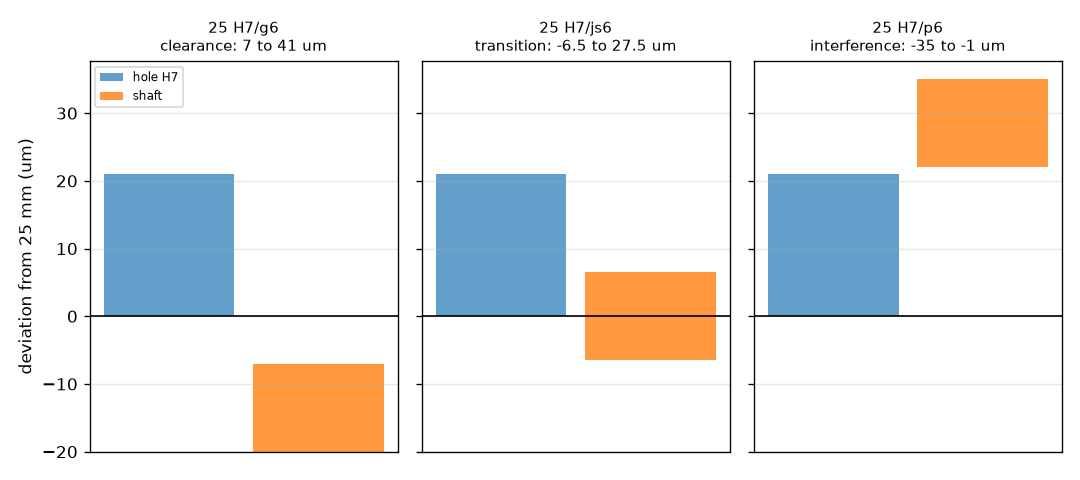
\includegraphics[width=0.85\linewidth]{figures/s02_fit_zones.png}\\\small Tolerance zones of three fits of a 25 mm shaft in an H7 hole: clearance (g6), transition (js6) and interference (p6).\end{center}

\subsection*{E. Worked example}
Compute the limits and the clearance of the fit 25 H7/g6, then the worst-case gap of a four-part stack: a housing of 40.00 +-0.10 mm holding three plates of 10.00 +-0.05, 12.00 +-0.05 and 15.00 +-0.08 mm.
\begin{enumerate}[nosep]
\item Hole H7: EI = 0, ES = +21 um, so the hole is 25.000 to 25.021 mm.
\item Shaft g6: es = -7 um and the width is IT6 = 13 um, so ei = -7 - 13 = -20 um; the shaft is 24.980 to 24.993 mm.
\item Smallest clearance = EI - es = 0 - (-7) = 7 um (0.007 mm = 25.000 - 24.993). Largest = ES - ei = 21 - (-20) = 41 um (0.041 mm = 25.021 - 24.980).
\item The minimum is not negative, so 25 H7/g6 is a clearance fit. Check: 41 - 7 = 34 um = IT7 + IT6 = 21 + 13.
\item Stack: nominal gap = 40.00 - 10.00 - 12.00 - 15.00 = 3.00 mm. Worst-case tolerance = 0.10 + 0.05 + 0.05 + 0.08 = 0.28 mm, so the gap lies between 2.72 and 3.28 mm. Trying all 16 corners gives the same two values.
\end{enumerate}
\textbf{Answer.} 25 H7/g6 has a clearance of 7 to 41 um; the stack gap is 3.00 mm with worst-case limits 2.72 and 3.28 mm.

\subsection*{F. Questions}
\begin{enumerate}[nosep]
\item \textbf{Conceptual.} Why is a fit with minimum clearance 0 (such as H7/h6) still called a clearance fit, and what separates a transition fit from an interference fit?
\item \textbf{Numerical.} Find the smallest and largest clearance of 25 H7/h6, using IT6 = 13 um, IT7 = 21 um and es = 0 for h. Sanity check: what must their difference be?
\item \textbf{Graph and simulation interpretation.} In the zone figure, how far above the top of the H7 hole zone does the p6 shaft zone start? What does that mean for assembly?
\item \textbf{Design and optimisation challenge.} Design: select a fit from H7/g6, H7/h6, H7/js6 and H7/p6 for (a) a sliding bearing that needs at least 5 um and at most 45 um of clearance and (b) a gear that must stay on its shaft with interference in every build and at most 40 um of it. Give the clearance limits that justify your choice, and say what is wrong with the others.
\end{enumerate}

\section{Session 3: Statistical stack-up, capability and cost}

\subsection*{A. Real-world problem}
Worst-case stack-up is safe but expensive: it makes every part so accurate that it assumes all of them can be at their worst limit in the same assembly. With five independent parts that is very unlikely. Statistical tolerancing accepts a tiny, calculated fraction of out-of-tolerance assemblies in exchange for looser, cheaper parts. But what if the machine drifts? Can a design that passes on paper fail a few percent of builds? And given the cost of each part, how should the tolerance be shared out?

\subsection*{B. Concept and theory}
We take a part tolerance t as plus or minus three standard deviations of the process (sigma = t / 3), so that about 99.7 percent of that part is inside its tolerance. For independent parts, variances add, so the gap has sigma\_gap = sqrt(sum of sigma\_i squared) and a plus or minus three sigma tolerance of sqrt(sum of t\_i squared): the root-sum-square, RSS. It is never larger than the worst-case sum. With specification limits LSL and USL, the capability index is Cp = (USL - LSL) / (6 sigma), and Cpk = min(USL - mu, mu - LSL) / (3 sigma) also penalises a mean mu that is off-centre. A common guideline is Cp of at least 1.33, which puts the limits four sigma from the centre. For a normal distribution, the fraction outside the limits is Phi((LSL - mu)/sigma) + 1 - Phi((USL - mu)/sigma), where Phi(z) = (1 + erf(z / sqrt 2)) / 2. In the illustrative cost model the cost of part i is k\_i / t\_i, so halving the tolerance doubles the cost; minimising the total cost for a given RSS gap tolerance (Lagrange multipliers) gives t\_i proportional to the cube root of k\_i. All of this is a simplified model: real parts may be skewed or correlated, and real cost curves differ.

\begin{itemize}[nosep]
\item t\_i: tolerance (plus or minus) of part i, taken as 3 sigma (mm)
\item sigma\_i, sigma\_gap: standard deviation of part i and of the gap (mm)
\item LSL, USL: lower and upper specification limits of the gap (mm)
\item mu: mean of the gap (mm)
\item Cp, Cpk: process capability indices (no unit)
\item k\_i: illustrative cost coefficient of part i (cost = k\_i / t\_i) (cost unit x mm)
\item drift: shift of every process centre, in multiples of its own sigma (no unit)
\end{itemize}

\begin{equation*}
\sigma_i = \frac{t_i}{3},\qquad \sigma_{\mathrm{gap}} = \sqrt{\sum_i \sigma_i^2},\qquad t_{\mathrm{RSS}} = \sqrt{\sum_i t_i^2}
\end{equation*}

\begin{equation*}
C_p = \frac{USL - LSL}{6\sigma},\qquad C_{pk} = \frac{\min(USL-\mu,\ \mu-LSL)}{3\sigma}
\end{equation*}

\begin{equation*}
P_{\mathrm{out}} = \Phi\!\left(\frac{LSL-\mu}{\sigma}\right) + 1 - \Phi\!\left(\frac{USL-\mu}{\sigma}\right),\qquad \Phi(z) = \tfrac12\left(1+\mathrm{erf}\frac{z}{\sqrt2}\right)
\end{equation*}

\begin{equation*}
\min \sum_i \frac{k_i}{t_i}\ \text{ with }\ \sum_i t_i^2 = T^2 \ \Rightarrow\ t_i \propto k_i^{1/3}
\end{equation*}

\begin{center}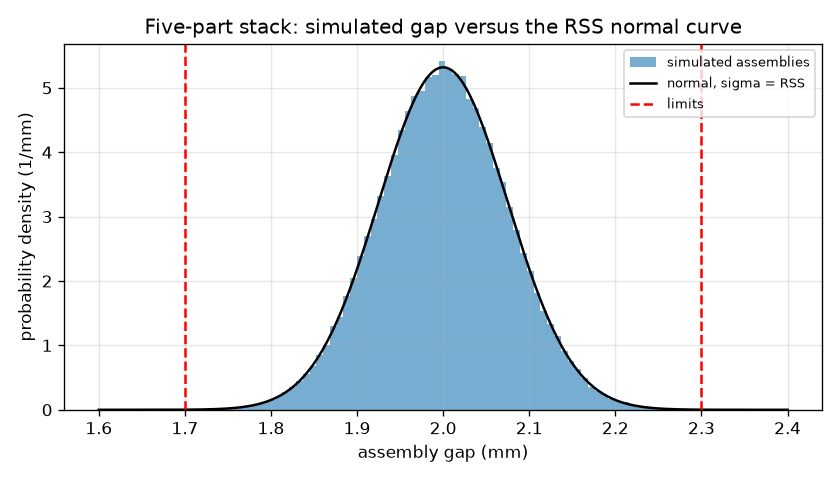
\includegraphics[width=0.85\linewidth]{figures/s03_gap_histogram.png}\\\small 200000 simulated five-part assemblies: the histogram follows the RSS normal curve, with limits four sigma away.\end{center}

\subsection*{E. Worked example}
Five independent parts each have a tolerance of +-0.10 mm and the gap must stay within 2.00 +-0.30 mm. Find the worst-case and RSS gap tolerances, sigma, Cp and the fraction out of tolerance for a centred process.
\begin{enumerate}[nosep]
\item Worst case: 5 x 0.10 = 0.500 mm. That is far outside +-0.30 mm, so a worst-case design would fail the requirement.
\item RSS: sqrt(5 x 0.10\textasciicircum{}2) = 0.10 x sqrt 5 = 0.224 mm (0.2236). This is inside +-0.30 mm.
\item Sigma of the gap = 0.2236 / 3 = 0.0745 mm.
\item Cp = (2.30 - 1.70) / (6 x 0.0745) = 0.60 / 0.447 = 1.34, just above the 1.33 guideline.
\item The limits are 0.30 / 0.0745 = 4.02 sigma away, so the fraction out is 2 x Phi(-4.02) = 5.7e-5, that is 0.0057 percent, about 1 assembly in 17500. Monte Carlo and corner enumeration check the sigma and the corners (1.50 to 2.50 mm).
\end{enumerate}
\textbf{Answer.} Worst case +-0.500 mm, RSS +-0.224 mm, sigma 0.0745 mm, Cp 1.34, about 0.0057 percent of assemblies out of tolerance.

\subsection*{F. Questions}
\begin{enumerate}[nosep]
\item \textbf{Conceptual.} Why is the root-sum-square tolerance never larger than the worst-case sum, and what assumption lets us use it? What do we pay for the smaller number?
\item \textbf{Numerical.} A gap has limits 1.70 and 2.30 mm and a process with mean 2.10 mm and sigma 0.075 mm. Find Cp and Cpk and say what the difference means.
\item \textbf{Graph and simulation interpretation.} In the drift graph, what happens to the fraction out when the drift grows from 0 to 1 sigma for the allocated tolerances? Read it at 0.5 and 1.0 sigma.
\item \textbf{Design and optimisation challenge.} Design: five parts get equal tolerances. Find the equal tolerance t that gives Cp = 1.33 (four sigma) for a gap of 2.00 +-0.30 mm using RSS, and compare its cost, using k = 3.0, 0.4, 1.0, 0.2 and 0.6, with the equal worst-case design. Is the worst-case design makeable if no process can hold better than +-0.05 mm?
\end{enumerate}

\section{Real-world mini-project}
\textbf{Allocate tolerances to a five-part assembly at minimum cost.} A housing (52.00 mm) holds four stacked parts (10.00, 12.00, 15.00 and 13.00 mm), leaving a gap of 2.00 mm that must stay within 2.00 +-0.30 mm. The process must be capable: Cp of at least 1.33 for the gap, with every part tolerance at least +-0.05 mm. The parts have illustrative cost coefficients k = 3.0, 0.4, 1.0, 0.2 and 0.6 (cost = k / tolerance). Use \texttt{allocate\_rss} and \texttt{cost} from Session 3 to find the cheapest allocation, compare it with equal tolerances and with a worst-case design, and test the result by Monte Carlo simulation.

\section{The path ahead}
\begin{enumerate}[nosep]
\item \textbf{Session 4: Parts that are not normal.} A stack simulator that draws each part from a normal, a uniform or a skewed distribution.
\item \textbf{Session 5: Watch for drift with a control chart.} A control chart with three-sigma limits on subgroups of five, driven by a slowly drifting simulated process.
\item \textbf{Session 6: Allocate with standard IT grades.} An allocator that picks an IT grade for each part from a table and minimises the illustrative cost.
\item \textbf{Session 7: Design that survives drift.} A design search that adds a drift allowance and reports the cheapest allocation that still passes.
\item \textbf{Session 8: Stacks in two dimensions.} A stack where one part is tilted, with each tolerance weighted by the sine or cosine of its angle.
\end{enumerate}

\section{Answers and hints}

\subsection*{Session 1}
\begin{enumerate}[nosep]
\item \textbf{Conceptual.} Hint: Think about what a machine can and cannot hold, and read the definition of 'in tolerance'. Solution: No process produces an exact size every time (tool wear, temperature, measurement error), so the drawing states how far from the ideal the size may be. The limits are the largest and smallest acceptable sizes. A part exactly on a limit is still in tolerance, because the limits themselves are allowed.
\item \textbf{Numerical.} Hint: clearance = hole - pin; then compare each size with its limits. Solution: Clearance = 10.04 - 9.95 = 0.09 mm. The pin is between 9.93 and 9.98 and the hole between 10.00 and 10.05, so both are in tolerance. The value 0.09 mm lies between the smallest (0.02 mm) and largest (0.12 mm) clearance, as it must.
\item \textbf{Graph and simulation interpretation.} Hint: Which limits does the smallest clearance use, and do they move when tol changes? Solution: The smallest clearance uses the hole lower limit (10.00) and the pin upper limit (9.98); neither depends on tol, so it stays at 0.02 mm. The largest uses the hole upper limit and the pin lower limit, and both move outwards by tol, so it equals 0.02 + 2 tol. At tol = 0.10 mm it is 0.02 + 0.20 = 0.22 mm.
\item \textbf{Design and optimisation challenge.} Hint: Set the largest clearance 0.02 + 2 tol to at most 0.10 mm. Solution: 0.02 + 2 tol \textless{}= 0.10 gives tol \textless{}= 0.04 mm. At tol = 0.04 the clearance range is 0.02 to 0.10 mm: always assembles and never exceeds the wobble limit. A smaller tolerance (for example 0.02 mm, clearance 0.02 to 0.06 mm) also works but parts must be made more accurately, which costs more; that trade-off returns in Session 3.
\end{enumerate}

\subsection*{Session 2}
\begin{enumerate}[nosep]
\item \textbf{Conceptual.} Hint: Look at the classification rule: which clearance limit must be non-negative or non-positive? Solution: A clearance fit is one where the minimum clearance is not negative, so no pair can interfere; for H7/h6 the minimum is exactly 0 and the largest shaft just equals the smallest hole. In an interference fit the maximum clearance is not positive, so every pair has interference. In a transition fit the minimum is negative and the maximum positive, so some pairs have clearance and others interference.
\item \textbf{Numerical.} Hint: h6 spans -13 to 0 um. Apply EI - es and ES - ei. Solution: Shaft h6: es = 0, ei = -13 um. Minimum = EI - es = 0 - 0 = 0 um. Maximum = ES - ei = 21 - (-13) = 34 um. The difference 34 um equals IT7 + IT6 = 21 + 13, as it must.
\item \textbf{Graph and simulation interpretation.} Hint: The hole zone ends at +21 um; the p6 zone starts at its lower deviation. Solution: The p6 zone starts at +22 um, which is 1 um above the top of the hole zone (+21 um). Even the smallest shaft is 1 um bigger than the largest hole, so every pair has interference (1 to 35 um): a light press fit that needs force or heating to assemble.
\item \textbf{Design and optimisation challenge.} Hint: Compute the minimum and maximum clearance of each fit; then test them against the requirements. Solution: H7/g6: 7 to 41 um, H7/h6: 0 to 34 um, H7/js6: -6.5 to +27.5 um, H7/p6: -35 to -1 um. (a) Only g6 satisfies 5 to 45 um; h6 can have 0 um (no oil film) and js6 can interfere. (b) Only p6 has interference in every build (1 to 35 um, within 40 um); h6 and g6 never interfere and js6 only sometimes. Assumption: the requirements are illustrative; real press fits also check hole stress and torque.
\end{enumerate}

\subsection*{Session 3}
\begin{enumerate}[nosep]
\item \textbf{Conceptual.} Hint: Think about how likely it is that all parts are at their worst limit together, and about independence. Solution: The square root of a sum of squares is at most the sum itself, so RSS \textless{}= sum. It applies when the parts vary independently and roughly normally, so large errors of different parts tend to cancel. The price is a small, calculated fraction of assemblies that may fall outside the gap tolerance, and the need for the processes to stay centred and stable.
\item \textbf{Numerical.} Hint: Cp = (USL - LSL) / (6 sigma); Cpk uses the nearer limit. Solution: Cp = 0.60 / (6 x 0.075) = 1.33. Cpk = min(2.30 - 2.10, 2.10 - 1.70) / (3 x 0.075) = 0.20 / 0.225 = 0.89. The spread would be good enough (Cp 1.33) but the process is off-centre, so the nearer limit is only 2.7 sigma away and Cpk is below 1. Sanity check: Cpk \textless{}= Cp always.
\item \textbf{Graph and simulation interpretation.} Hint: The graph compares the erf curve with the simulation dots. Solution: At no drift it is 6.3e-5, essentially zero; at 0.5 sigma it is about 0.17 percent; at 1.0 sigma it is about 3.1 percent (3.08 percent by erf, 3.06 by simulation). The curve is very steep: a drift of one sigma in every part turns a safe design into one that rejects about 1 assembly in 32.
\item \textbf{Design and optimisation challenge.} Hint: RSS target = 0.30 / 1.33 = 0.225 mm; t = target / sqrt 5. Worst case: t = 0.30 / 5. Solution: RSS: t = 0.225 / sqrt 5 = 0.101 mm, cost = sum of k / t = 5.2 / 0.1006 = 51.68. Worst case: t = 0.060 mm, cost = 5.2 / 0.06 = 86.67, 68 percent more. Both are makeable at +-0.05 mm. Trade-off: the statistical design is cheaper but relies on independent, centred, normal processes; the worst-case design needs no assumptions.
\end{enumerate}

\section{How to join}
Read \texttt{CONTRIBUTING.md} in the repository, then pick an issue labelled \texttt{good first issue}. Repository: \url{https://github.com/KrunalPanchal1995/opentolerance}

\end{document}
